\documentclass[tikz,border=2pt]{standalone}
\usepackage{amsmath}
\usetikzlibrary{arrows.meta}
\begin{document}
% (s,S) cost recursion for s = 0, S = 2, lead time 1, demand D in {0,1,2} w.p. 1/4, 1/2, 1/4,
% h = 1, b = 4, K = 6: self-loops with f_0 = 1/4, V(s,1) = 23/3, V(s,2) = 76/9; stopping set {x <= 0}.
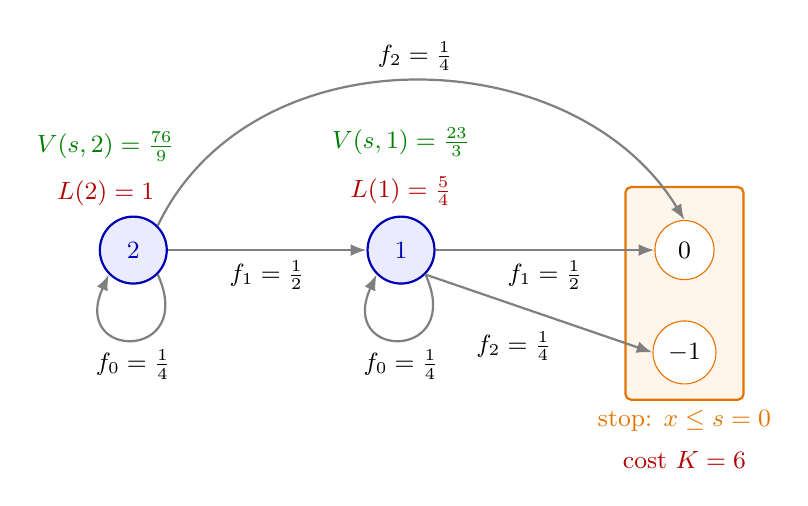
\begin{tikzpicture}[font=\small, >={Latex[length=2mm]},
  st/.style={draw=blue!70!black, thick, circle, fill=blue!8, minimum size=0.85cm, text=blue!70!black}]
  \node[st] (x2) at (0,0) {$2$};
  \node[st] (x1) at (3.4,0) {$1$};
  % stopping set
  \node[draw=orange!90!black, thick, fill=orange!8, rounded corners=2pt, minimum width=1.5cm, minimum height=2.7cm] (stop) at (7.0,-0.55) {};
  \node[draw=orange!90!black, circle, minimum size=0.75cm, fill=white] (x0) at (7.0,0) {$0$};
  \node[draw=orange!90!black, circle, minimum size=0.75cm, fill=white] (xm) at (7.0,-1.3) {$-1$};
  \node[orange!90!black, anchor=north] (sl) at (stop.south) {stop: $x\leq s=0$};
  \node[red!70!black, anchor=north] at (sl.south) {cost $K=6$};
  % self-loops below the states: zero demand
  \draw[->, thick, gray] (x2.south east) .. controls +(0.5,-1.1) and +(-0.5,-1.1) .. (x2.south west) node[pos=0.5, below, black] {$f_0=\tfrac{1}{4}$};
  \draw[->, thick, gray] (x1.south east) .. controls +(0.5,-1.1) and +(-0.5,-1.1) .. (x1.south west) node[pos=0.5, below, black] {$f_0=\tfrac{1}{4}$};
  % transitions
  \draw[->, thick, gray] (x2) -- (x1) node[pos=0.5, below, black] {$f_1=\tfrac{1}{2}$};
  \draw[->, thick, gray] (x1) -- (x0) node[pos=0.5, below, black] {$f_1=\tfrac{1}{2}$};
  \draw[->, thick, gray] (x1.south east) -- (xm.west) node[pos=0.6, below left, black] {$f_2=\tfrac{1}{4}$};
  \draw[->, thick, gray] (x2.north east) .. controls +(1.2,2.5) and +(-1.4,2.3) .. (x0.north) node[pos=0.5, above, black] {$f_2=\tfrac{1}{4}$};
  % running costs and values above the states
  \node[red!70!black, anchor=south] (l2) at ([xshift=-0.35cm]x2.north) {$L(2)=1$};
  \node[green!50!black, anchor=south] at (l2.north) {$V(s,2)=\tfrac{76}{9}$};
  \node[red!70!black, anchor=south] (l1) at (x1.north) {$L(1)=\tfrac{5}{4}$};
  \node[green!50!black, anchor=south] at (l1.north) {$V(s,1)=\tfrac{23}{3}$};
\end{tikzpicture}
\end{document}
